\documentclass{article}
\usepackage{amsmath}
\usepackage{amsthm}
\usepackage{amssymb}
\usepackage{enumerate}
\usepackage{graphicx}

\begin{document}
    \title{Exercise 2.3}
    \author{Wang Yue from Elite Class}
    \date{\today}

    \maketitle

    \section*{Evaluate the limit and justify each step by indicating the appropriate Limit Law(s).}

    \subsection*{9. $\lim_{x \to 2}\frac{2x^2+1}{3x-2}$}

    $$
    \begin{aligned}
        \lim_{x\to 2}\frac{2x^2+1}{3x-2} &= \sqrt{\lim_{x \to 2}\frac{2x^2+1}{3x-2}} \\
        &= \sqrt{\frac{\lim_{x \to 2}2x^2+1}{\lim_{x \to 2}3x-2}} \\
        &= \sqrt{\frac{9}{4}} \\
        &= \frac{3}{2}
    \end{aligned}
    $$

    \section*{Evaluate the limit, if it exists.}

    \subsection*{14. $\lim_{x \to -1}\frac{x^2-4x}{x^2-3x-4}$}

    $$
    \begin{aligned}
        \lim_{x \to -1}\frac{x^2-4x}{x^2-3x-4} &= \lim_{x \to -1}{x(x-4)}{(x-4)(x+1)} \\
        &= \lim_{x \to -1}\frac{x}{x + 1} \\
        &= \lim_{x \to -1}(1 - \frac{1}{x + 1})
    \end{aligned}
    $$
    $\because$ when $x \to -1^-$, $\frac{1}{x+1} \to -\infty$, when $x \to -1^+$, $\frac{1}{x+1} \to \infty$

    $\therefore \lim_{x \to -1}\frac{1}{x+1}$ does not exist. 

    $\therefore \lim_{x \to -1}\frac{x^2-4x}{x^2-3x-4}$ does not exist.

    \subsection*{18. $\lim_{h \to 0}\frac{(2 + h)^3 - 8}{h}$}

    $$
    \begin{aligned}
        \lim_{h \to 0}\frac{(2 + h)^3 - 8}{h} &= \lim_{h \to 0}\frac{(h^2 + 4h + 4)(h + 2)}{h} \\
        &= \lim_{h \to 0}\frac{h^3 + 6h^2 + 12h + 8 - 8}{h} \\
        &= \lim_{h \to 0}(h^2 + 6h + 12) \\
        &= \lim_{h \to 0}h^2 + \lim_{h \to 0}6h + \lim_{h \to 0}12 \\
        &= 12
    \end{aligned}
    $$

    \subsection*{22. $\lim_{u \to 2}\frac{\sqrt{4u + 1} - 3}{u - 2}$}
    
    $$
    \begin{aligned}
        \lim_{u \to 2}\frac{\sqrt{4u + 1} - 3}{u - 2} &= \lim_{u \to 2}\frac{4u + 1 - 3^2}{(u - 2)(\sqrt{4u + 1} + 3)} \\
        &= \lim_{u \to 2}\frac{4(u - 2)}{(u - 2)(\sqrt{4u + 1} + 3)} \\
        &= \lim_{u \to 2}\frac{4}{\sqrt{4u + 1} + 3} \\
        &= \frac{4}{3 + 3} = \frac{2}{3}
    \end{aligned}
    $$

    \subsection*{25. $\lim_{t \to 0}\frac{\sqrt{1 + t} - \sqrt{1 - t}}{t}$}

    $$
    \begin{aligned}
        \lim_{t \to 0}\frac{\sqrt{1 + t} - \sqrt{1 - t}}{t} &= \lim_{t \to 0}\frac{(\sqrt{1 + t} - \sqrt{1 - t})(\sqrt{1 + t} + \sqrt{1 - t})}{t(\sqrt{1 + t} + \sqrt{1 - t})} \\
        &= \lim_{t \to 0}\frac{1 + t - 1 + t}{t(\sqrt{1 + t} + \sqrt{1 - t})} \\
        &= \lim_{t \to 0}\frac{2}{\sqrt{1 + t} + \sqrt{1 - t}} \\
        &= \frac{2}{\lim_{t \to 0}{\sqrt{1 + t} + \sqrt{1 - t}}} \\
        &= \frac{2}{1 + 1} \\
        &= 1
    \end{aligned}
    $$

    \subsection*{29. $\lim_{t \to 0}(\frac{1}{t\sqrt{1 + t}} - \frac{1}{t})$}
    
    $$
    \begin{aligned}
        \lim_{t \to 0}(\frac{1}{t\sqrt{1 + t}} - \frac{1}{t}) &= \lim_{t \to 0}\frac{1 - \sqrt{1 + x}}{x\sqrt{1+x}} \\
        &= \lim_{t \to 0}\frac{1 - (1 + x)}{x\sqrt{1+x}(1 + \sqrt{1 + x})} \\
        &= \lim_{t \to 0}\frac{-1}{\sqrt{1 + x}(1 + \sqrt{1+x})} \\
        &= \lim_{t \to 0}\frac{-1}{1 + x + \sqrt{1 + x}} \\
        &= \frac{-1}{1 + 0 +1} \\
        &= -\frac 1 2
    \end{aligned}
    $$

    \subsection*{39. Prove that $\lim_{x \to 0}x^4\cos{\frac 2 x} = 0$}

    \begin{proof}
        $\because -1 < \cos \frac{2}{x} < 1$

        $\therefore -x^4 < x^4\cos \frac 2 x < x^4$

        $\because \lim_{x \to 0}-x^4 = \lim_{x \to 0}x^4 = 0$

        $\therefore$ by the squeeze theorem, $$\lim_{x \to 0}x^4\cos \frac 2 x = 0$$
    \end{proof}

    \subsection*{40. Prove that $\lim_{x \to 0^+} \sqrt{x} e^{\sin(\pi/x)} = 0$}

    \begin{proof}
        $\because -1 < \sin(\frac{\pi}{x}) < 1$

        $\therefore \frac{\sqrt x}{e} < \sqrt x e^{\sin(\frac{\pi}{x})} < e\sqrt x$

        $\because \lim_{x \to 0}\frac{\sqrt{x}}{e} = \lim_{x \to 0}e\sqrt{x} = 0$

        $\therefore$ by the squeeze theorem, $$\lim_{x \to 0}\sqrt x e^{\sin(\frac{\pi}{x})} = 0$$
        
    \end{proof}

    \subsection*{47. The $sigsum$(or sign)$function$, denoted by sgn, is defined by $$sgn x = \left\{ \begin{array}{ll} -1 & \textrm{if x < 0} \\ 0 & \textrm{if x = 0} \\ 1 & \textrm{if x > 0} \end{array} \right.$$}

    (a) Sketch the graph of this function.

    The graph of the function is shown below.

    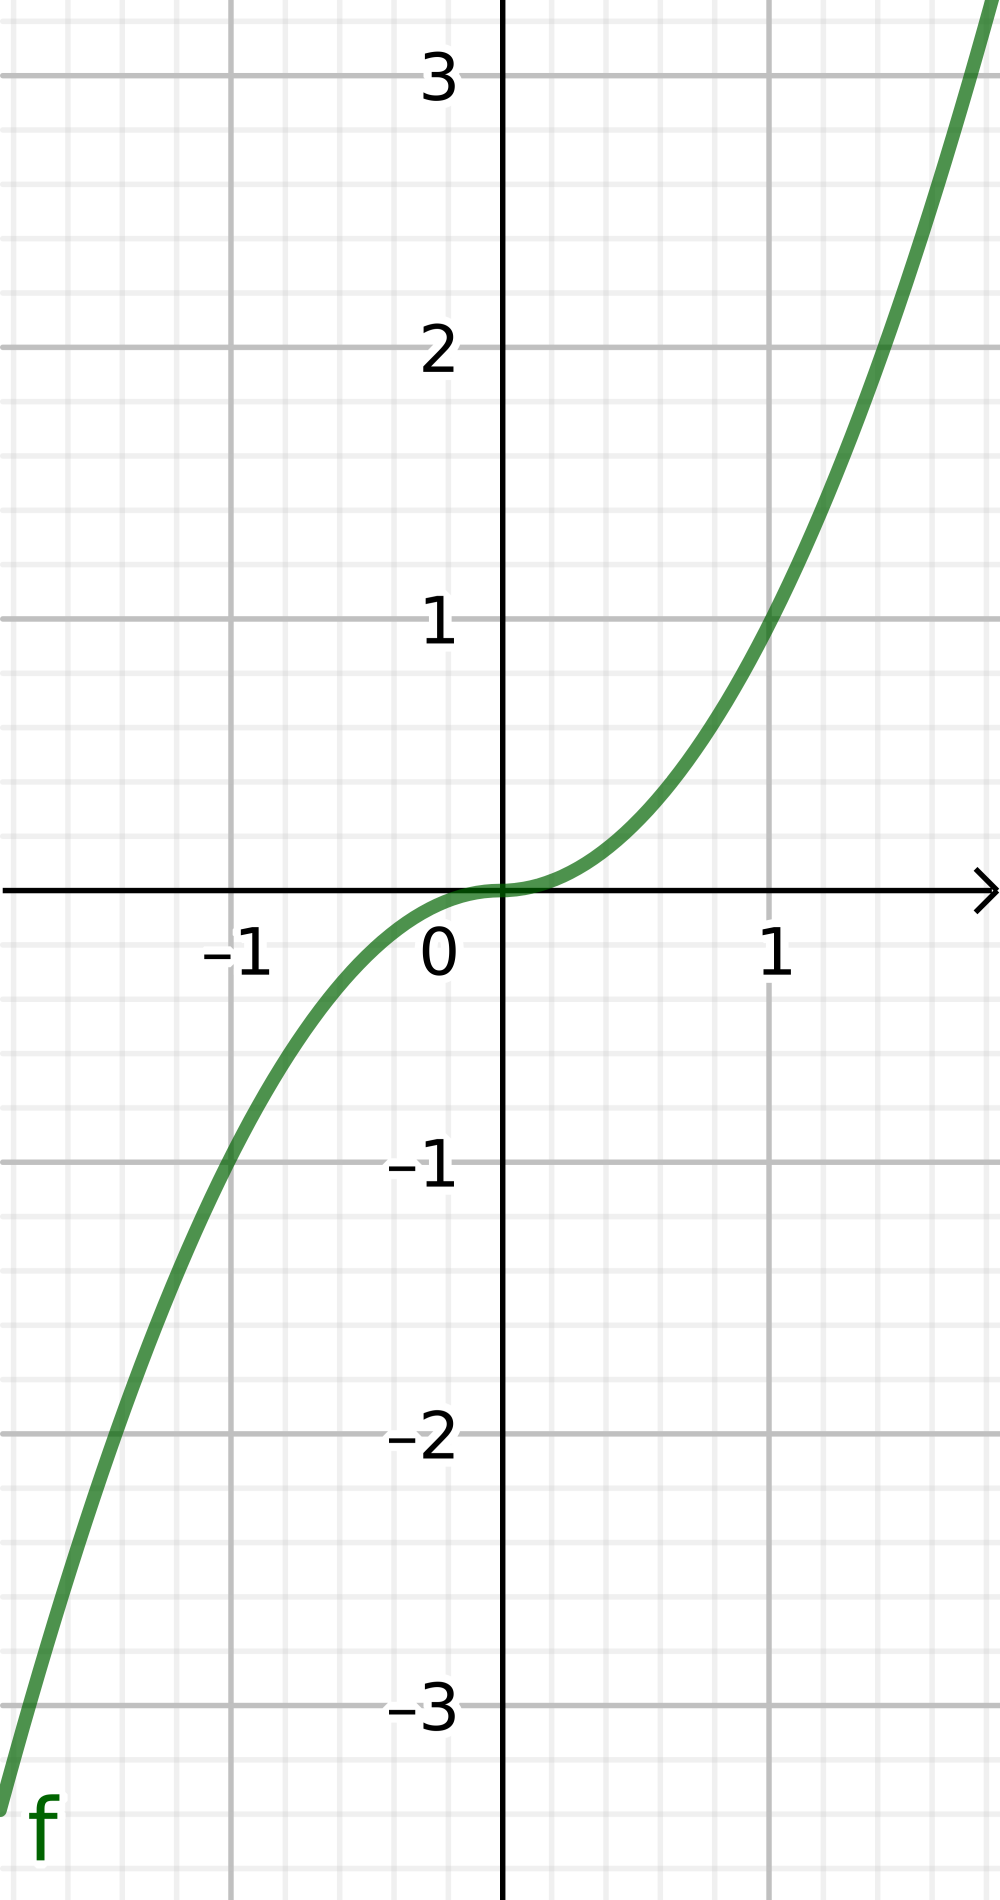
\includegraphics[scale = 1.7]{geogebra-export.png}

    (b) Find each of the following limits or explain why it does not exist.

    \begin{enumerate}
        \item $\lim_{x \to 0^+}$ sgn x
        The limit is $1$.
        \item $\lim_{x \to 0^-}$ sgn x
        The limit is $-1$.
        \item $\lim_{x \to 0}$ sgn x
        By the answer of two problems above, we know that $$\lim_{x \to 0^+} sgn x \not = \lim_{x \to 0^-} sgn x$$

        So $\lim_{x \to 0} sgn x$ does not exist.
        \item $\lim_{x \to 0}$ |sgn x|
        By the answer of two problems above, we know that $$|\lim_{x \to 0^+} sgn x| = |\lim_{x \to 0^-} sgn x| = 1$$

        So $\lim_{x \to 0}|sgn x|$ = 1
    \end{enumerate}

    \subsection*{57. If $\lim_{x \to 1}\frac{f(x) - 8}{x - 1} = 10$, find $\lim_{x \to 1}f(x)$}

    $$
    \begin{aligned}
        \lim_{x \to 1}f(x) &= 10(\lim_{x \to 1}(x - 1)) + 8 \\
        &= 8
    \end{aligned}
    $$

    \subsection*{58. If $\lim_{x \to 0}\frac{f(x)}{x^2} = 5$, find the following limits.}

    \begin{enumerate}[a.]
        \item $\lim_{x \to 0}f(x)$
        $$
        \begin{aligned}
            \lim_{x \to 0}f(x) &= \lim_{x \to 0}\frac{f(x)}{x^2} * \lim_{x  \to 0}x^2 \\
            &= 5 \times \lim_{x \to 0}x^2 \\
            &= 0
        \end{aligned}
        $$
        \item $\lim_{x \to 0}\frac{f(x)}{x}$

        $$
        \begin{aligned}
            \lim_{x \to 0}\frac{f(x)}{x} &= \lim_{x \to 0}\frac{f(x)}{x^2} * \lim_{x \to 0}x \\
            &= 5 \times 0 \\
            &= 0
        \end{aligned}
        $$
    \end{enumerate}


    
    \subsection*{59. If $$f(x) = \left\{ \begin{array}{ll} x^2 & \textrm{if x is rational} \\ 0 & \textrm{if x is irrational}  \end{array} \right.$$ prove that $\lim_{x \to 0}f(x) = 0$}

    \begin{proof}
        $\forall \epsilon > 0, \exists \delta = \sqrt{\epsilon}$

        if $0 < |x - 0| < \delta$, then we can start our discussion.

        \begin{enumerate}
            \item If $\delta \in Q$, then $$|f(x) - 0| < |f(\delta) - 0| = |\delta^2| = \epsilon$$
            \item If $\delta \not \in Q$, so $\exists \delta_0 \in Q $ and $ \delta_0 < \delta$, so $$|f(x) - 0| < |f(\delta_0)| = \delta_0^2 < \delta^2 = \epsilon$$
        \end{enumerate}

        So no matter whether $\delta \in Q$, $\lim_{x \to 0}f(x) = 0$

    \end{proof}

    \subsection*{60. Show by means of an example that $\lim_{x \to a}[f(x) + g(x)]$ may exist even though neither $\lim_{x \to a}f(x)$ nor $\lim_{x \to a}g(x)$ exists.}
    \begin{proof}
        Let $f(x) = \frac{1}{x - a}$, $g(x) = -\frac{1}{x - a}$

        Obviously, both the limit of $f(x)$ and $g(x)$ do not exist when $x$ approach $a$.

        But $$f(x) + g(x) = \frac{1}{x - a} - \frac{1}{x - a} = 0$$

        So $\lim_{x \to a}[f(x) + g(x)]$ exists, and the value is $0$.
    \end{proof}

    \subsection*{61. Show by means of an example that $\lim_{x \to a}[f(x)g(x)]$ may exist even though neither $\lim_{x \to a}f(x)$ nor $\lim_{x \to a}g(x)$ exists.}
    \begin{proof}
        Let $f(x) = e^{\frac{1}{x - a}}$, $g(x) = e^{-\frac{1}{x - a}}$

        Obviously both the limit of $f(x)$ and $g(x)$ do not exist when $x$ approach $a$.

        But $$f(x)g(x) = e^{\frac{1}{x - a} - \frac{1}{x - a}} = e^0 = 1$$

        So $\lim_{x \to a}[f(x)g(x)]$ exists, and the value is $1$.
    \end{proof}

    \subsection*{62. Evaluate $\lim_{x \to 2}\frac{\sqrt{6 -x } - 2}{\sqrt{3 - x} - 1}$}
    $$
    \begin{aligned}
        \lim_{x \to 2}{\frac{\sqrt{6 -x} - 2}{\sqrt{3 - x} - 1}} &= \lim_{x \to 2}\frac{6 - x - 4}{(\sqrt{3 - x} - 1)(\sqrt{6 - x} + 2)} \\
        &= \lim_{x \to 2}\frac{(2 - x)(\sqrt{3 - x} + 1)}{(\sqrt{6 - x} + 2)(3 - x - 1)} \\
        &= \lim_{x \to 2}\frac{\sqrt{3 - x} + 1}{\sqrt{6 - x} + 2} \\
        &= \frac{2}{4} = \frac{1}{2}
    \end{aligned}
    $$

\end{document}